% Compile with XeLaTeX, TeXLive 2013 or more recent
\documentclass{beamer}

% Base packages
\usepackage{fontspec}
\usepackage{xunicode}
\usepackage{xltxtra}

\usepackage{amsfonts}
\usepackage{amsmath}
\usepackage{longtable}
\usepackage{csquotes}
\usepackage{standalone}
\usepackage{bytefield}

% Setup fonts
\newfontfamily\russianfont{CMU Serif}
\setromanfont{CMU Serif}
\setsansfont{CMU Sans Serif}
\setmonofont{CMU Typewriter Text}

% Setup Russian hyphenation. NOTE: this declaration *must* come after fontspec's font declarations,
% or a mysterious (but harmless in other respects) error "Improper `at' size (0.0pt), replaced by 10pt." would appear.
\usepackage{polyglossia}
\defaultfontfeatures{Scale=MatchLowercase, Mapping=tex-text}

\setdefaultlanguage[spelling=modern]{russian} % for polyglossia
\setotherlanguage{english} % for polyglossia

% Vector drawings
\usepackage{tikz}
% \usetikzlibrary{shapes, calc, arrows, fit, positioning, decorations, patterns, decorations.pathreplacing, chains, snakes}
\usetikzlibrary{shapes, calc, arrows, decorations.markings, decorations.pathreplacing, decorations.pathmorphing, decorations, patterns, chains, snakes, backgrounds, positioning, fit, shadows}
% \usepackage[siunitx]{circuitikz}

% Be able to insert hyperlinks
\usepackage{hyperref}
\hypersetup{colorlinks=true, linkcolor=black, filecolor=black, citecolor=black, urlcolor=blue , pdfauthor=Grigory Rechistov <grigory.rechistov@phystech.edu>, pdftitle=Курс «Программное моделирование вычислительных систем»}
% \usepackage{url}

% Misc optional packages
\usepackage{underscore}
\usepackage{amsthm}

% A new command to mark not done places
\newcommand{\todo}[1][Напиши меня]{{\color{red}TODO\ #1}}
\newcommand{\abbr}{\textit{англ.}\ }

\title{Двоичная трансляция}
\subtitle{Курс «Программное моделирование вычислительных систем»}
\subject{Курс «Программное моделирование вычислительных систем»}

\author[]{Григорий Речистов \\ \small{\href{mailto:grigory.rechistov@phystech.edu}{grigory.rechistov@phystech.edu}}}
\date{\today}
\pgfdeclareimage[height=0.5cm]{ilab-logo}{../ilab-noletters.png}
\logo{\pgfuseimage{ilab-logo}}

\typeout{Copyright 2015 Grigory Rechistov}

\usetheme{Berlin}
\setbeamertemplate{navigation symbols}{}%remove navigation symbols

\begin{document}

\begin{frame}
    \maketitle
\end{frame}

\begin{frame}
    \tableofcontents
\end{frame}


\begin{frame}{На (поза)прошлой лекции}
\begin{itemize}
\item Интерпретаторы — медленная шутка
\item Рассмотренные улучшения основаны на повторном использовании уже полученных результатов
\item Существуют устоявшиеся идиомы для представления моделируемого архитектурного состояния
\end{itemize}
\end{frame}

\begin{frame}{Вопросы}
\begin{itemize}
% \item Определите термин «декодирование» \pause
\item Сколько бит в машинном слове? \pause
\item Что лучше — MMIO или PIO?\pause
\item Может ли архитектура быть и не little, и не big-endian?
\end{itemize}

\end{frame}

% «»

\begin{frame}{Что удалось соптимизировать в интерпретаторе}
\begin{itemize}
\item \textbf<1>{Fetch} \only<1>{$\leftarrow$ оптимизировано}
\item \textbf<1>{Decode} \only<1>{$\leftarrow$ оптимизировано}
\item \textbf<2>{Execute} \only<2>{$\rightarrow$ осталось соптимизировать}
\item \textbf<2>{Writeback} \only<2>{$\rightarrow$ осталось соптимизировать}
\item \textbf<2>{Advance PC} \only<2>{$\rightarrow$ осталось соптимизировать}
\end{itemize}

\end{frame}

\section{Интерпретация, компиляция, трансляция}

\begin{frame}{Интерпретация и трансляция в языках высокого уровня}
\begin{itemize}
\item BASIC, CPython, Shell\dots
    \begin{itemize}
    \item Прочитать строку — распознать команды — исполнить
    \item Медленно работает, но больше «интерактивности»
    \end{itemize}
\item Fortran, C, Pascal\dots
    \begin{itemize}
    \item Первый проход: распознавание команд языка и преобразование их в машинный код
    \item Второй проход: исполнение машинного кода
    \end{itemize}
\end{itemize}
\end{frame}

\begin{frame}{Двоичная трансляция}
\begin{itemize}
\item Входной язык — гостевой машинный код
\item Целевой язык — хозяйский машинный код
\item ДТ — перевод кода гостевой программы, записанной в гостевой ISA, в эквивалентный код в терминах хозяйской ISA
\item Ради чего: многократное исполнение результатов трансляции
\end{itemize}
\end{frame}

\begin{frame}{Статическая и динамическая ДТ}
\begin{itemize}
    \item \textit{Статическая} трансляция исполняется заранее, до исполнения первой инструкции
    \item Результат статической трансляции сохраняется на диске
    \item \textit{Динамическая} трансляция происходит непосредственно во время симуляции
    \item Результат динамической трансляции хранится в памяти
    \item Динамическая трансляция чередуется с исполнением генерированного кода
\end{itemize}

\end{frame}

\begin{frame}[fragile]{Фазы динамической ДТ}
\centering
\input{./../../simbook/metoda/drawings/dynamic-bt}
\end{frame}

\section{Шаблонная трансляция}

\begin{frame}{Алгоритм 1: шаблонная трансляция}
\begin{tikzpicture}[font=\scriptsize, >=latex, node distance=2.cm]

\node[draw, double copy shadow={shadow xshift=3pt,shadow yshift=-3pt}, fill=white] (decode) {decode_t};
\node[rectangle split, rectangle split parts=4, draw, right=of decode, anchor=text west, minimum width=1.8cm] (templates-raw) {Шаблон 1\nodepart{two} Шаблон 2\nodepart{three} Шаблон 3\nodepart{four} Шаблон 4};


\node[rectangle split, rectangle split parts=4, draw, right=of templates-raw, minimum width=1.8cm] (templates) {Капсула 1\nodepart{two} Капсула 2\nodepart{three} Капсула 3\nodepart{four} Капсула 4};

\node[draw, above=1cm of templates-raw, align=left] (md) {Кодировки и смещения\\операндов хозяйских\\инструкций};

\draw[->] (decode) -- (templates-raw.text west) node[midway, above]{\tiny Выбор шаблонов};
\draw[->] (templates-raw) -- (templates);
\coordinate[above=0.5cm of templates] (junction);
\draw[->] (decode) |- (junction) -- (templates) node[pos=0, above]{\tiny Подстановка аргументов};
\draw[] (md) |- (junction);

\end{tikzpicture}

\end{frame}

\begin{frame}[fragile]{Алгоритм 1: шаблонная трансляция}
\begin{tiny}
\begin{itemize}
    \item start_addr — гостевой адрес начала кода
    \item start_buf — хозяйский буфер
\end{itemize}
\end{tiny}

\begin{verbatim}
translate(start_addr, start_buf) {
    PC = start_addr; bufptr = start_buf;
    while (!enough) {
        instr = fetch(PC);
        (opcode, operands) = decode(instr);
        (template, length) = templates[opcode];
        memcpy(bufptr, template, length);
        patch_operands(bufptr, operands);
        PC += instr_length;
        bufptr += length;
    }
    memcpy(bufptr, glue_capsule, glue_length);
}
\end{verbatim}
\end{frame}

\begin{frame}[fragile]{Алгоритм 1: исполнение}

\begin{verbatim}
execute(start_buf) {
    load_simulated_state();
    goto start_buf;
}
\end{verbatim}
\pause
или
\begin{verbatim}
typedef void (*fblock)(void);
execute(start_buf) {
    load_simulated_state();
    ((fblock)start_buf)();
}
\end{verbatim}

\end{frame}

\begin{frame}{Капсула}

\begin{small}
\begin{tabular}{p{0.45\textwidth}p{0.45\textwidth}}
Гостевой код, Intel~64 (64 бит) & Хозяйский код, IA-32 (32 бит)
\end{tabular}
\end{small}

\vfill

\centering
\input{./../../simbook/metoda/drawings/capsule}\pause

Вопрос: что из семантики \texttt{ADDQ} забыто в описании капсулы?
\end{frame}

\begin{frame}{Подстановка аргументов в капсулу}

{\ttfamily\small
{\sffamily Регистры:}

\begin{tabular}{ll}  
c5 f4 58 c\textcolor{red}{8}  &    vaddps \textcolor{red}{\%ymm0},\%ymm1,\%ymm1 \\
c5 f4 58 c\textcolor{red}{9}  &    vaddps \textcolor{red}{\%ymm1},\%ymm1,\%ymm1 \\
c5 f4 58 c\textcolor{red}{f}  &    vaddps \textcolor{red}{\%ymm7},\%ymm1,\%ymm1 \\\pause
c4 c1 74 58 c\textcolor{red}{8} &  vaddps \textcolor{red}{\%ymm8},\%ymm1,\%ymm1 \\
c4 c1 74 58 c\textcolor{red}{f} &  vaddps \textcolor{red}{\%ymm15},\%ymm1,\%ymm1 \\
c5 f4 58 c8  &    vaddps \%ymm0,\%ymm1,\%ymm1 \\
c5 ec 58 d0  &    vaddps \%ymm0,\%ymm2,\%ymm2 \\
c5 c4 58 f8  &    vaddps \%ymm0,\%ymm3,\%ymm3 \\\pause
c4 e1 74 58 c8 &  vaddps \%ymm0,\%ymm1,\%ymm1 \# Мнемоника та же!\\
\end{tabular}

\pause
{\sffamily Литералы:}
\begin{tabular}{ll}
67 c7 85 \textcolor{blue}{00 01 00 00} \textcolor{green}{dd cc bb aa}   & movl \textcolor{green}{\$0xaabbccdd},\textcolor{blue}{0x100}(\%ebp)
\end{tabular}
} % \ttfamily

\end{frame}

\section{Трансляция с IR}

\begin{frame}{Алгоритм 2: JIT. Генерация IR}
\centering
\begin{tikzpicture}[font=\small, >=latex]

\node[rectangle split, rectangle split parts=2, draw, double copy shadow={shadow xshift=3pt,shadow yshift=-3pt}, fill=white] (sr) {Эмуляционная процедура\nodepart{two} С (подмножество)};
\node[rectangle split, rectangle split parts=2, draw, below=1cm of sr, double copy shadow={shadow xshift=3pt,shadow yshift=-3pt}, fill=white] (template) {Шаблон\nodepart{two} IR: байткод+SSA};
\draw[->] (sr) -- (template) node[midway, right] {SR-компилятор};

% \node[above = of sr] (compile-time) {При компиляции};
\end{tikzpicture}
\end{frame}

\begin{frame}{Алгоритм 2: JIT. Стадия симуляции}
\begin{tikzpicture}[font=\scriptsize, >=latex, node distance=1.cm]

% \node[] (run-time) {При симуляции};

\node[draw, double copy shadow={shadow xshift=3pt,shadow yshift=-3pt}, fill=white] (decode) {decode_t};
\node[rectangle split, rectangle split parts=4, draw, right=of decode, anchor=text west, minimum width=1.8cm] (templates) {Шаблон 1\nodepart{two} Шаблон 2\nodepart{three} Шаблон 3\nodepart{four} Шаблон 4};
\draw[->] (decode) -- (templates.text west);

\node[draw, below=0.5cm of templates, minimum height=2cm, align=left, minimum width=1.8cm] (opt-template) {Шаблон\\блока};
\draw[->] (templates) -- (opt-template) node[midway, right] {Оптимизация};

\node[rectangle split, rectangle split parts=3, align=left, draw, below=0.5cm of opt-template, double copy shadow={shadow xshift=3pt,shadow yshift=-3pt}, fill=white] (md) {Машинное описаниe (md)\nodepart{two} Байткод → машинный код\nodepart{three} Определения хоз. регистров};

\coordinate[right=2.5cm of opt-template] (junction);

\node[draw, right=1cm of junction, rectangle split, rectangle split parts=2,] (host-code) {Блок трансляции\nodepart{two} Хозяйский машинный код};

\draw[->] (md) -| node[pos=0.5, right, align=left] {Распределение регистров\\Кодогенерация} (junction) -- (host-code);
\draw[] (opt-template) -- (junction);

\end{tikzpicture}
    
\end{frame}

\begin{frame}{Оптимизации}
\centering
\input{./../../simbook/metoda/drawings/bt-optimization}

\end{frame}

\begin{frame}{Связь между блоками трансляции}
\centering
\input{./../../simbook/metoda/drawings/bb-translation}
\end{frame}

\begin{frame}{Почему оптимизации при ДТ затруднительны}

\begin{itemize}
    \item В отличие от ЯВО, машинный код содержит меньше информации об исходном алгоритме
    \item Нельзя делать многие предположения, необходимые для компиляторных оптимизаций, без нарушения корректности
    \item В случае динамической ДТ оптимизации ограничены длительностью их работы
\end{itemize}\pause

\begin{itemize}
\item Адреса переменных — их нет
\item Границы процедур — их нет
\item Адреса переходов — известна только часть из них
\end{itemize}


\end{frame}

\section{Трудности ДТ}

\begin{frame}{Самомодифицирующийся код (self modifying code)}
\centering
\begin{tikzpicture}[font=\scriptsize, >=latex]
    \node (guest) {Гость};
    \node[right=3cm of guest] (host) {Хозяин};

    \node[draw, minimum width = 1.5cm, minimum height = 0.5cm, below =0.5cm of guest] (gi1) {};
    \node[draw, minimum width = 1.5cm, minimum height = 0.5cm, below = 0cm of gi1] (gi2) {};
    \node[draw, minimum width = 1.5cm, minimum height = 0.5cm, below = 0cm of gi2] (gi3) {};

    \node[draw, minimum width = 1.5cm, minimum height = 1cm, below =0.5cm of host] (hi1) {};
    \node[draw, minimum width = 1.5cm, minimum height = 2cm, below = 0cm of hi1] (hi2) {};
    \node[draw, minimum width = 1.5cm, minimum height = 1.5cm, below = 0cm of hi2] (hi3) {};

    \draw[->] (gi1.east) to (hi1.west);
    \draw[->] (gi2.east) to (hi2.west);
    \draw[->] (gi3.east) to (hi3.west);
    \pause
    \node[draw = red, minimum width = 2cm, cross out] at (gi3) {};
    \draw[->, dashed, thick, ] (hi2.center) .. controls (2, -4) and (-3, -3) .. (gi3.west) node[pos=0.5, below] {Запись в память};
    
\end{tikzpicture}

\end{frame}

\begin{frame}{Обнаружение кода 1}
\begin{itemize}
    \item Найти границы инструкций
    \item Отличить код от данных
\end{itemize}
\centering
\begin{tikzpicture}[font=\scriptsize, >=latex]
    \node (guest) {Гость};
    \node[right=3cm of guest] (host) {Хозяин};

    \node[draw, minimum width = 2cm, minimum height = 0.5cm, below =0.5cm of guest] (gi1) {};
    \node[draw, minimum width = 2cm, minimum height = 0.5cm, below = 0cm of gi1] (gi2) {};
    \node[draw, minimum width = 2cm, minimum height = 0.5cm, below = 0cm of gi2] (gi3) {};
    \node[draw, minimum width = 2cm, minimum height = 0.5cm, below = 0cm of gi3] (gjmp) {jmp \$pc-6};

    \node[draw, minimum width = 1.5cm, minimum height = 1cm, below =0.5cm of host] (hi1) {};
    \node[draw, minimum width = 1.5cm, minimum height = 1.5cm, below = 0cm of hi1] (hi2) {};
    \node[draw, minimum width = 1.5cm, minimum height = 1cm, below = 0cm of hi2] (hi3) {};
    \node[draw, minimum width = 1.5cm, minimum height = 0.5cm, below = 0cm of hi3] (hi4) {jmp \$pc-?};

    \draw[->] (gi1.east) to (hi1.west);
    \draw[->] (gi2.east) to (hi2.west);
    \draw[->] (gi3.east) to (hi3.west);

    \draw[->] (gjmp.south) |- ([xshift=-2cm, yshift=-0.5cm]gjmp.south) |- (gi1.south west);
    
\end{tikzpicture}

\end{frame}

\begin{frame}{Обнаружение кода 2}
\begin{center}
\input{./../../simbook/metoda/drawings/byte-shift}
\end{center}

По этой причине статическое пре-декодирование не всегда возможно
\end{frame}

\begin{frame}{Опережающая трансляция}
\centering
\begin{tikzpicture}[>=latex, font=\small, align=left]
    \node[draw] (tb100) {Блок трансляции\\0x100 → 0xa000};
    \node[above=of tb100] (pred) {\dots};
    \node[draw, below= of tb100] (tb110) {Блок трансляции\\0x110 → 0xa100};
    \node[draw, left=of tb110.south west, anchor=north east] (tb130) {Блок трансляции\\0x130 → 0xa200};
    \node[below=of tb130] (cont) {\dots};
    \draw[->] (tb100) -- (tb110);
    \draw[->] (tb110.220) |- (tb130);
    \draw[->] (tb130) -- (cont);
    \draw[->] (pred) -- (tb100);
    
    \uncover<1-2>{\node[draw=black!30, right=of tb110.south east, anchor=north west, text=black!30] (notb200) {Нет трансляции\\0x200 → ?};}
    \uncover<2>{\draw[->, very thick] (pred) -- (tb100.center) -- (tb110.center) |- (notb200);}

    \uncover<3>{\node[draw, right=of tb110.south east, anchor=north west, cloud, aspect=2]  (in-progress) {Трансляция\\0x200};}

    \uncover<4->{\node[draw, right=of tb110.south east, anchor=north west] (tb200) {Блок трансляции\\0x200 → 0xb000};}
    \uncover<4->{\draw[->] (tb110) |- (tb200);}

%     \uncover<4>{;}
    \uncover<5>{\draw[->, very thick] (pred) -- (tb100.center) -- (tb110.center) |- (tb200);}
    
\end{tikzpicture}

\end{frame}

\begin{frame}{Трансляция горячего кода}
\only<1>{Исполнение 1: интерпретация с трассированием}
\only<2>{Исполнение $N$: обнаружение «горячих» участков трассы}
\only<3>{Трансляция трассы в блоки}
\only<4>{Подстановка новых блоков в трассу}

\vfill

\centering
\begin{tikzpicture}[>=latex, font=\small]
\uncover<1,2,4>{
    \coordinate (pred);
    \node[draw, below=0.5cm of pred, minimum height=1cm] (tb1) {};
    \coordinate[below=0.25cm of tb1] (jp1);
    \coordinate[below=0.25cm of jp1] (jp2);
    \node[draw, minimum height=1cm, left=of jp2, anchor=north] (tb2) {};
}
\uncover<1-3>{
    \node[draw, minimum height=1cm, right=of jp2, anchor=north] (tb3) {};
    \node[draw, minimum height=0.75cm, below=0.5cm of tb3] (tb4) {};
}
\uncover<2>{\node[draw, fill=red, minimum height=1cm, right=of jp2, anchor=north] (tb3-hot) {};}
\uncover<2>{\node[draw, fill=red, minimum height=0.75cm, below=0.5cm of tb3] (tb4-hot) {};}

    \coordinate[below=of tb2] (post2);
    \coordinate[below=of tb4] (post4);
\uncover<1,2>{\draw[->] (tb4) -- (post4);}
\uncover<1,2,4>{
    \draw[->] (pred) -- (tb1);
    \draw[->] (tb1.south) -- (jp1) -| (tb2);
    \draw[->] (tb1.south) -- (jp1) -| (tb3);
    \draw[->] (tb2) -- (post2);
}
\uncover<1,2,3>{
    \draw[->] (tb3) -- (tb4);
    \draw[->] (tb4.south) -- ([yshift=-0.25cm]tb4.south) -| ([xshift=1cm, yshift=0.25cm]tb3.north) -| (tb3);
}

\uncover<3>{
    \node[draw, fill=green, minimum height=0.5cm, minimum width=0.5cm, right=3cm of tb3, anchor=north] (tb5-temp) {};
    \path (tb3.south) -- (tb5-temp) node[pos=0.7] {\huge $\Rightarrow$};   
}

\uncover<4>{
    \node[draw, fill=green, minimum height=0.5cm, minimum width=0.5cm, right=of jp2, anchor=north] (tb5) {};
    \draw[->] (tb5) -- (tb4);
}    
\end{tikzpicture}
\end{frame}

\section{Заключение}

\begin{frame}{Итоги}
\begin{itemize}
\item Интерпретация, компиляция, трансляция
\item Двоичная трансляция
\item Статическая и динамическая трансляция
\item Шаблон, капсула
\item Промежуточное представление
\item Самомодифицирующийся код
\item Обнаружение кода
\item Сложности оптимизации кода при ДТ
\end{itemize}
\end{frame}


\begin{frame}[allowframebreaks]{Литература}
\begin{thebibliography}{99}
    \bibitem{vms} Jim Smith and Ravi Nair. Virtual Machines: Versatile Platforms for Systems and Processes. Morgan Kaufmann - 2005
    \begin{center}
    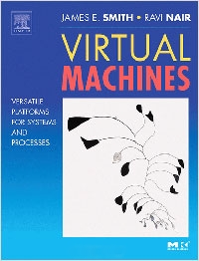
\includegraphics[height=0.5\textheight]{./vm-book}
    \end{center}
    
    \bibitem{qemu} Fabrice Bellard. QEMU, a Fast and Portable Dynamic Translator \url{http://www.usenix.org/publications/library/proceedings/usenix05/tech/freenix/full_papers/bellard/bellard.pdf}
    \bibitem{fx32} Anton Chernoff and Ray Hookway. {DIGITAL FX!32} Running 32-Bit x86 Applications on {Alpha} {NT} \url{http://www.usenix.org/publications/library/proceedings/usenix-nt97/full_papers/chernoff/chernoff.pdf}
    \bibitem{ia32el} Leonid Baraz [et al.] IA-32 Execution Layer: a Two-Phase Dynamic Translator Designed to Support IA-32 Applications on Itanium®-Based Systems. \url{http://www.microarch.org/micro36/html/pdf/goldenberg-IA32ExecutionLayer.pdf}
\end{thebibliography}
\end{frame}

% The final "thank you" frame 

\begin{frame}{На следующей лекции}
\centering

Ещё быстрее! Прямое исполнение
\vfill


\includegraphics[width=0.5\textwidth]{./moar}
\end{frame}

\begin{frame}

{\huge{Спасибо за внимание!}\par}

\vfill

Слайды и материалы курса доступны по адресу \url{http://is.gd/ivuboc} % http://atakua.doesntexist.org/wordpress/simulation-course-russian/

\vfill

\tiny{\textit{Замечание}: все торговые марки и логотипы, использованные в данном материале, являются собственностью их владельцев. Представленная здесь точка зрения отражает личное мнение автора, не выступающего от лица какой-либо организации.}

\end{frame}

\end{document}


\begin{frame}{Время компиляции и время исполнения}
\todo новое
\end{frame}

\begin{frame}{Переключение таблиц}
\todo новое
\end{frame}

